\documentclass[letterpaper, 10 pt, conference]{ieeeconf}
\IEEEoverridecommandlockouts % This command is only needed if
% you want to use the \thanks command

\overrideIEEEmargins % Needed to meet printer requirements.

% See the \addtolength command later in the file to balance the column
% lengths on the last page of the document
\usepackage{microtype}
% The following packages can be found on http:\\www.ctan.org
% \usepackage{graphics} % for pdf, bitmapped graphics files
% \usepackage{epsfig} % for postscript graphics files
% \usepackage{mathptmx} % assumes new font selection scheme installed
% \usepackage{times} % assumes new font selection scheme installed
% \usepackage{amsmath} % assumes amsmath package installed
% \usepackage{amssymb} % assumes amsmath package installed

\usepackage[pdftex,pdfauthor={anonymous},pdftitle={6.867 Pset 1}]{hyperref}
\hypersetup{colorlinks,linkcolor={green!50!black},citecolor={green!50!black},urlcolor={blue!80!black}}
\makeatletter \let\NAT@parse\undefined \makeatother
% \usepackage[square,comma,sort&compress]{natbib}
\usepackage[sort,compress]{cite}
\usepackage{graphicx} % more modern
\usepackage{amsfonts}
\usepackage{amsmath,soul}
\usepackage{color}
\usepackage[font=small]{subcaption}
\usepackage{balance}
\usepackage[font=small]{caption}
%\usepackage{subfigure,balance}
%\usepackage[colorlinks=true]{hyperref}
%\usepackage{subcaption,balance}
%\usepackage{algorithm} \usepackage[noend]{algorithmic}
\usepackage[linesnumbered,ruled,vlined]{algorithm2e}
\usepackage{multirow}

% from bjorn:
\usepackage{xfrac}
\usepackage{mathtools}
\usepackage{bm}


\DeclareMathOperator*{\argmin}{\arg\!\min}
\DeclareMathOperator*{\argmax}{\arg\!\max}
\usepackage{tabulary}
\newcolumntype{K}[1]{>{\centering\arraybackslash}p{#1}}


\newtheorem{definition}{Definition}
\newtheorem{assumption}{Assumption} \newtheorem{theorem}{Theorem}
\newtheorem{lemma}{Lemma}
\newtheorem{corollary}[theorem]{Corollary}

\title{\LARGE \bf 6.867: Homework 2}

\author{Anonymous authors}

% \usepackage[usenames]{color}
%\DeclareMathOperator*{\argmin}{arg\,\!min}
%\DeclareMathOperator*{\argmax}{arg\,\!max}
\usepackage[svgnames]{xcolor} \definecolor{DarkGreen}{rgb}{0,0.5,0}
\definecolor{DarkRed}{rgb}{0.75,0,0}

\usepackage[authormarkuptext=name,addedmarkup=bf,authormarkupposition=left]{changes}
%\usepackage[final]{changes} %Use this to hide all comments.
\definechangesauthor[name={M.~E.}, color={red}]{me}
\setremarkmarkup{(#2)}

%\newcommand{\mXX}[1]{{\color{DarkRed} \bf XX #1 XX\ }}
\newcommand{\mXX}[1]{\added[id=ml,remark={}]{#1}}
\newcommand{\sXX}[1]{\added[id=sc,remark={}]{#1}}
%\newcommand{\XX}[1]{{\bf \color{red} XX #1 XX}}
\newcommand{\XX}[1]{\added[id=jh,remark={}]{#1}}
\newcommand{\jmXX}[1]{\added[id=jm,remark={}]{#1}}
\newcommand{\meXX}[1]{\added[id=me,remark={}]{#1}}



\newcommand{\jsec}[1]{\marginpar{\fcolorbox{yellow}{yellow}{\parbox{0.7in}{\raggedright
        \color{blue} \tiny #1 }}}}
\newcommand{\hsec}[1]{\marginpar{\fcolorbox{yellow}{yellow}{\parbox{0.7in}{\raggedright
        \color{green} \tiny #1 }}}}
\newcommand{\jhmargin}[2]{{\color{orange}#1}\marginpar{\color{orange}\tiny\raggedright
    \bf [JH] #2}}


\usepackage{tikz,mathtools}
%\usepackage{cleveref}
\usepackage[capitalize]{cleveref}
\crefformat{equation}{(#2#1#3)}
\Crefformat{equation}{Equation~(#2#1#3)}
\Crefname{equation}{Equation}{Equations}

\newcommand{\inputTikZ}[2]{\scalebox{#1}{\input{#2}}}
\usetikzlibrary{shapes,positioning,automata,arrows,fit,backgrounds,calc}
\tikzstyle{block} = [draw, fill=blue!20, rectangle,minimum height=1em,
minimum width=2em] \tikzstyle{sum} = [draw, fill=blue!20, circle, node
distance=1cm] \tikzstyle{input} = [coordinate] \tikzstyle{output} =
[coordinate] \tikzstyle{pinstyle} = [pin edge={to-,thin,black}]
\usetikzlibrary{trees} \usetikzlibrary{decorations.pathmorphing}
\usetikzlibrary{decorations.markings}
\definecolor{darkgreen}{rgb}{0,0.5,0}
\definecolor{darkred}{rgb}{220,20,60}

\makeatletter
\renewcommand\paragraph{\@startsection{subsubsection}{4}{\z@}%
{0.25ex \@plus.5ex \@minus.2ex}%
{-.15em}%
{\normalfont\normalsize\itshape}}
\makeatother


\begin{document}

\maketitle
\thispagestyle{empty} \pagestyle{empty}

% %%%%%%%%%%%%%%%%%%%%%%%%%%%%%%%%%%%%%%%%%%%%%%%%%%%%%%%%%%%%%%%%%%%%%%%%%%%%%%%

\begin{abstract}
This is Machine Learning homework 2. Topics include Logistic Regression, SVM, Gaussian RBF Kernel, Pegasos, and classifying the MNIST dataset. All work has been done in Python.
\end{abstract}

%%%%%%%%%%%%%%%%%%%%%%%%%%%%%%%%%%%%%%%%%%%%%%%%%%%%%%%%%%%%%%%%%%%%%%%%%%%%%%%%
%!TEX root = main.tex
\section{Neural Networks} \label{sec:prob1}
In this problem, we implement a simple neural network in Python.
The network is trained with backpropogation and stochastic gradient descent.

\subsection{Part 1}
In this problem, we are mainly interested in classification tasks.
Thus, we pass the output of the final hidden layer through a softmax layer to generate a probability (outputs are positive and sum to 1) vector where each element $k$ is the probability of the input being in class $k$.

In general, the training objective is to minimize loss, so at each training step, we evaluate the loss function and compute its gradient, and then adjust the weights and biases in a direction to decrease loss according to the learning rate.
According to the backpropogation algorithm, the derivative of loss with respect to final activation is $\delta^L = Diag[f'(z)] \nabla_a loss$.
For this network with softmax output activation and cross-entropy loss function, we can compute $\delta^L = p(x) - y$, where p(x) is the predicted output for a particular training data point, $x$ in class $y$ (where p is also a function of the network weights, and other parameters).


\subsection{Part 2}
According to the Xavier Initialization, we can initialize weights to be a zero-mean Gaussian with variance [todo].
We initialize biases to zero, but if we initialize weights to zero as well, [todo].

\subsection{Part 3}
To add weight regularization, the objective function would look like:
\begin{equation}
J(w) = l(w) + \lambda(||w^{(1)}||^2_F + ||w^{(2)}||^2_F)
\end{equation}
The only change to the pseudo-code from the lecture notes would be an updated gradient term.
[todo]: gradient term.






%!TEX root = main.tex
\section{Convolutional Neural Network (CNN)} \label{sec:prob2}
In this section, we consider the Convolutional Neural Network (CNN) to perform artist identification on paintings.

\subsection{Part 1}
In a convolutional filter, if the first layer applies a 5x5 patch to the image to generate feature $Z_1$, and the second layer applies a 3x3 patch to feature $Z_1$ to generate feature $Z_2$, the receptive field of $Z_2$ (or dimensions of image that affect the node) is 7x7.
That is, a window of 49 neighboring pixels in the original image affects a single node at the output of the filter.
This allows the network to learn spatial features from the original image.
If the conv net becomes deeper (more layers), the network can use larger and more complex combinations of features/regions of the image.

\subsection{Part 2}
We are provided with a conv net (conv.py).
In total, there are [todo] layers: 2 convolutional layers, 1 flatten layer, and 2 dense layers.
The output is the maximum logit of the final dense layer.
[todo] confirm activation function. The hidden layer activation function is relu.
The loss function is softmax cross entropy with logits.
Loss is minimized with Gradient Descent (with a tunable learning rate parameter).

The provided network took about 45 seconds to train on a Macbook CPU.
After 1500 steps, the training accuracy is 87.4\%, and the validation accuracy is 57.5\%.
These numbers suggest overfitting, because the model does not generalize to unseen data very well.

\subsection{Part 3}
Next, we try two common techniques to improve CNN performance.
The first is early stopping.
Early stopping is when training is stopped after validation accuracy levels out, before it starts to decrease, to avoid overfitting.
In this scenario, \cref{fig:2_3_num_steps} shows that early stopping could be applied around step 1,000, because at this point, validation accuracy levels off but training accuracy continues to increase.
That behavior is a good indication of overfitting, because the model is improving on data it has seen, but not improving on data it has never seen. 
In addition to reducing overfitting and reducing model complexity, early stopping also has the benefit of shorter training time.

\begin{figure}
	\centering
	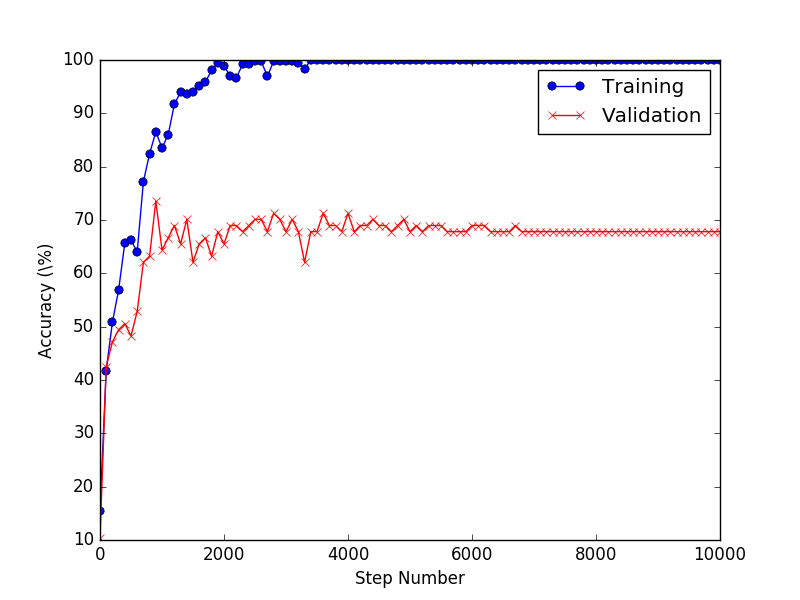
\includegraphics [trim=0 0 0 0, clip, angle=0, width=0.8\columnwidth,
	keepaspectratio]{figures/2_3_num_steps}
	\caption{Training and validation accuracy are plotted over 10,000 training steps. Validation performance levels off after 1,000 training steps, but training accuracy continues to increase. This behavior looks like overfitting, so training should be stopped early around step 1,000.} 
	\label{fig:2_3_num_steps} 
\end{figure}

The pooling layers seem to make no difference on performance.

\subsection{Part 4}
Finally, we use the network on a transformed version of the dataset.
Results in \cref{table_2_4} show that the performance is not the same for every transormation type.
For example, the original CNN only gets 10\% accuracy on inverted images, compared to 66.7\% on low contrast images (all relative to a 70.1\% accuracy on normal images).

\cref{table_2_4}'s columns show the original CNN, a CNN with Early Stopping and one with both Early Stopping and Max Pooling.
The results are not significantly different.
This aligns with the earlier observation that max pooling does not affect this problem much.
Early Stopping surprisingly didn't have much effect either.


\begin{table}[ht!]
\centering
\begin{tabular}{||c c c c||}  
 \hline
  & Regular & ES & ES \& Pooling \\
 Transformation & Val Acc (\%) & Val Acc (\%) & Val Acc (\%) \\ [0.3ex] 
 \hline\hline
 Normal & 65.5 & 70.1 & 69.0 \\ \hline
 Translated & 33.3 & 29.9 & 35.6 \\ \hline
 Brightened & 46.0 & 47.1 & 43.7 \\ \hline
 Darkened & 47.1 & 49.4 & 46.0 \\ \hline
 High Contrast & 62.1 & 63.2 & 58.6 \\ \hline
 Low Contrast & 66.7 & 66.7 & 67.8 \\ \hline
 Flipped & 42.5 & 41.4 & 44.8 \\ \hline
 Inverted & 8.0 & 10.3 & 12.6 \\ \hline
\end{tabular}
\caption{Accuracy of CNNs on transformed dataset, with Early Stopping (ES) and Max pooling.}
\label{table_2_4}
\end{table}




\section{Pegasos} \label{sec:prob3}
In this section, we use the Pegasos algorithm for soft-margin SVM binary classification of one of the 2D datasets.

\subsection{Part 1}
The Pegasos algorithm is a method to solve soft-margin SVM.
We implemented the algorithm according to the provided pseudocode, and added a bias term, $w_0$ that is incremented by $\eta_ty_i$ for misclassified sample $x_i$ each iteration.
The bias term is not penalized by the regularization.
The formulation solved by Pegasos is:
\begin{equation}\label{eq:svm_pegasos}
min_w \frac{\lambda}{2}||w||^2 + \frac{1}{N}\sum\limits_{i=1}^{N}max\{0,1-y_i(w^Tx_i)\}
\end{equation}

\subsection{Part 2}
The algorithm is applied to the same 2D dataset for several values of $\lambda$ ($\lambda = [2, 2^{-1}, 2^{-2}, 2^{-4}$), shown in~\cref{fig:3_2_lambdas}.
For large $\lambda$ (left), magnitude of $w$ is penalized heavily, so the decision boundary is not very accurate.
As $\lambda$ decreases, the regularization penalty becomes less dominant compared with accuracy, so the accuracy improves.
This intuition agrees with the objective function~\cref{eq:svm_pegasos}.

\begin{figure}
	\centering
	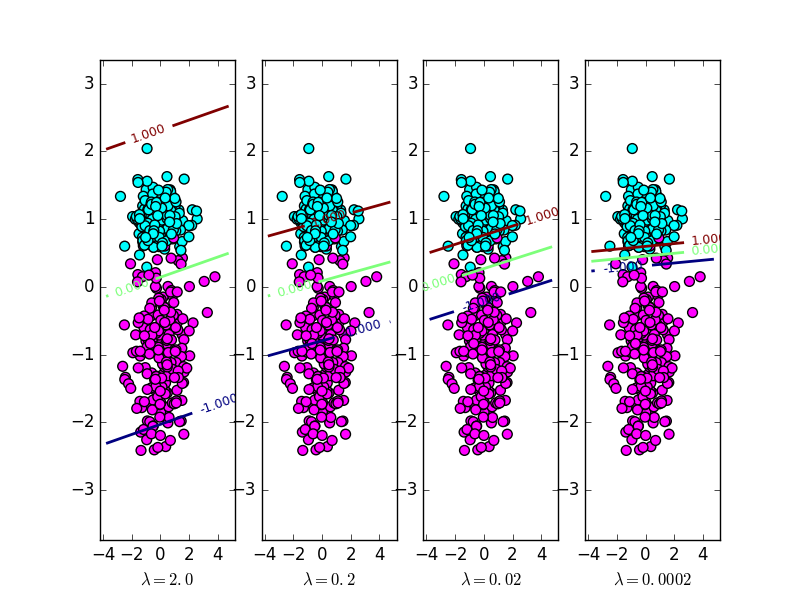
\includegraphics [trim=0 0 0 0, clip, angle=0, width=0.8\columnwidth,
	keepaspectratio]{figures/3_2_lambdas}
	\caption{The Pegasos algorithm is applied to the same dataset with four different regularization parameter values, $\lambda$. For large $\lambda$ (left), magnitude of $w$ is penalized heavily, so the decision boundary is not very accurate. As $\lambda$ decreases, the regularization penalty becomes less dominant compared with accuracy, so the accuracy improves.}
	\label{fig:3_2_lambdas} 
\end{figure}

\subsection{Part 3}
Next, we extended our implementation to handle a kernel matrix input, and tested it with a gaussian RBF kernel as in~\cref{sec:prob2}.
After learning $\alpha$, we predict the class of a new sample, $x_i$ by first calculating $c = \alpha \cdot K(X, x_i; \gamma)$, where $X$ is the entire training set and $\gamma$ is the Gaussian kernel bandwidth.
If $c > 0$, it's part of the positive class, otherwise it's the negative class.

\subsection{Part 4}
We tested our algorithm on multiple values of $\gamma$ with a fixed $\lambda=0.02$.
For large $\gamma$ (left), [todo], and the decision boundary overfits the data, evident in the decision boundary's jagged shape tracing around individual borderline samples.
As $\gamma$ decreases, the accuracy decreases, but the decision boundary is much less complicated.
This usually leads to better generalization to unseen data.

The number of support vectors decreases as $\gamma$ increases (192, 165, 10, 22).
This observation aligns with the decreasing complexity of the decision boundary, because each support vector affects the shape of the decision boundary.

These observations associated with increasing $\gamma$ match the trends seen in~\cref{sec:prob2} with increasing $C$.
Both implementations (Pegasos and SVM) are able to correctly classify the dataset.
Our Pegasos implementation runs much faster, making it easier to test with different parameters for increased performance.


\begin{figure}
	\centering
	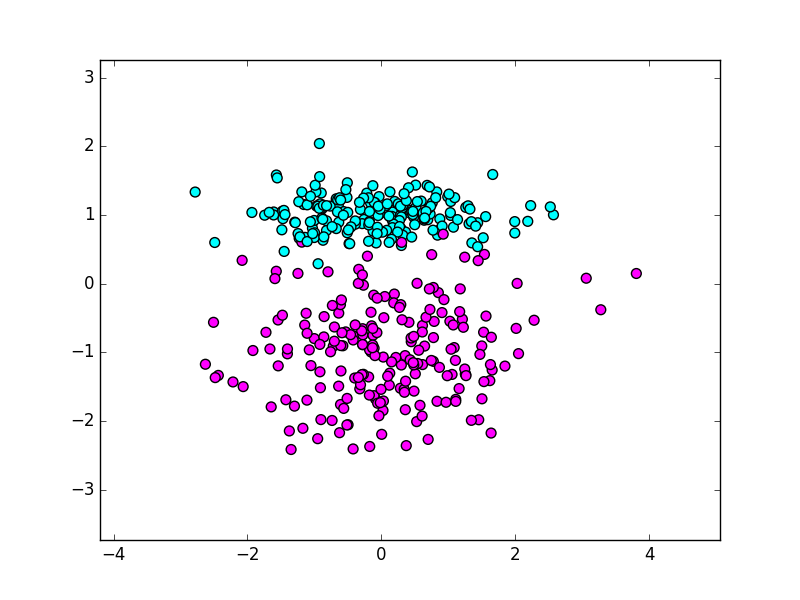
\includegraphics [trim=0 0 0 0, clip, angle=0, width=0.8\columnwidth,
	keepaspectratio]{figures/3_3_decisions}
	\caption{The Pegasos algorithm is applied to the same dataset with four different kernel bandwidth values, $\gamma = [2^2, 2^1, 2^0, 2^{-1}]$. For large $\gamma$ (left), [todo], and the decision boundary overfits the data. As $\gamma$ decreases, the accuracy decreases, but the decision boundary is much less complicated.}
	\label{fig:3_3_decisions} 
\end{figure}
\section{MNIST Dataset} \label{sec:prob4}
In this section, we use each of the algorithms to classify handwritten digits from the MNIST dataset.

\subsection{Part 1}
The MNIST dataset contains labeled, handwritten digits.
We split the dataset into multiple classification tasks, shown in the first column of~\cref{table_4_1}.
We also split it into training, validation, and testing sets.

We follow the typical procedure: train with many hyperparameters (C for $L_1$, $L_2$ for LR, and C for SVM), choose the hyperparameters that maximize performance on the validation set with lowest model complexity (low C), and report performance on the test set for the best hyperparameters.

The two classifiers here, Logistic Regression and Linear SVM, perform similarly on each classification task.
For all tasks, the training accuracy was better than the testing accuracy, as expected.

Normalization of the data did not make a large difference ($<\pm 1\%$) for these classifiers, and results presented are for non-normalized data.
The only significant difference after normalization was the size of regularization constant $C$; in all cases, normalization caused the optimal $C$ value to increase by a few orders of magnitude.
This is likely because the size of the data elements decreased, so the size of the learned weight vector increased, meaning a smaller regularization cost had to be applied for the same effect.

A couple misclassified digits are shown in~\cref{fig:misclassified}.
Some handwriting is very difficult even for humans to classify, so it makes sense that our learned classifiers are not perfect.

\begin{figure}\label{fig:misclassified}
    \centering
    \begin{subfigure}[b]{0.5\columnwidth}
        \centering
        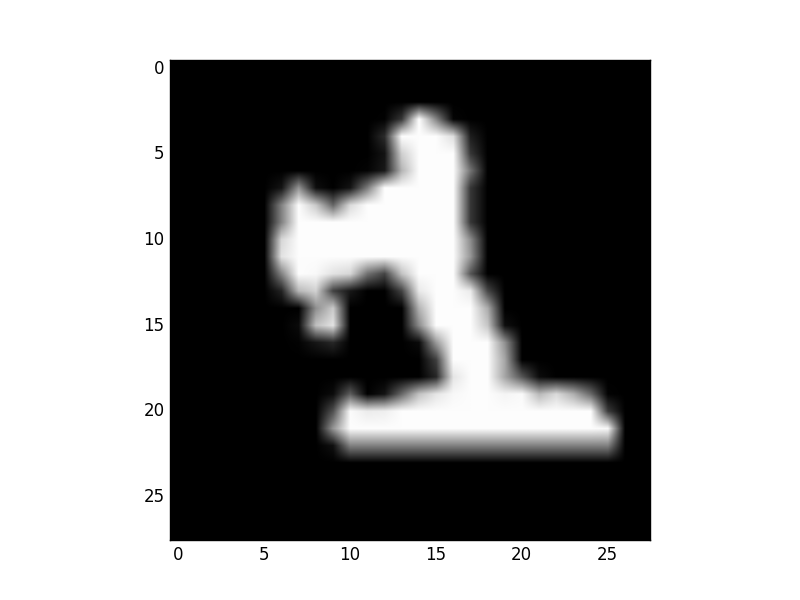
\includegraphics[height=1.2in]{figures/4_1_bad1}
        \caption{Misclassified 1}
    \end{subfigure}%
    ~ 
    \begin{subfigure}[b]{0.5\columnwidth}
        \centering
        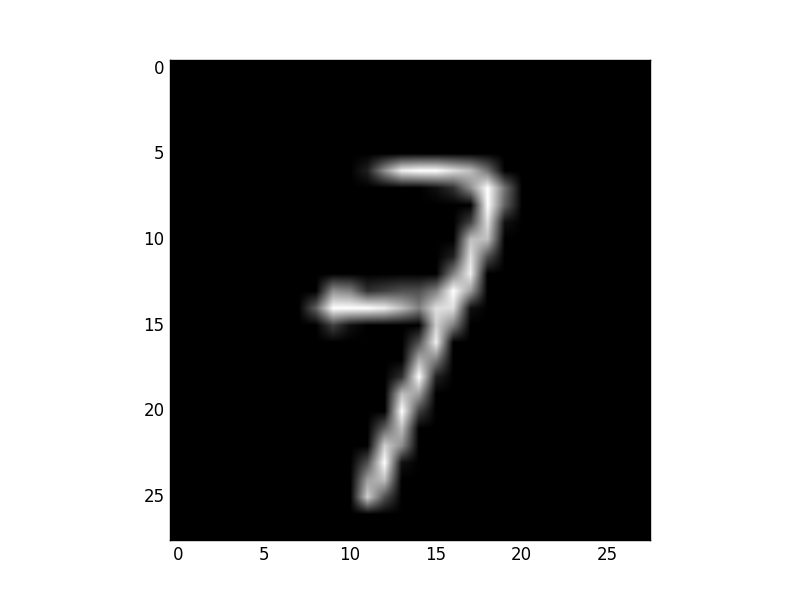
\includegraphics[height=1.2in]{figures/4_1_bad7}
        \caption{Misclassified 7}
    \end{subfigure}
    \caption{The MNIST dataset has some ambiguous entries, in accordance with real human handwriting, that are difficult to classify correctly.}
\end{figure}

\begin{table}[ht!]
\centering
\begin{tabular}{||c c c c c||}  
 \hline
 Dataset & LR Tr. & LR Test & SVM Tr & SVM Test \\ [0.3ex] 
 \hline\hline
 1 vs. 7 & 100.0 & 98.3 ($C=1$) & 100.0 & 98.7 ($C=0.2$) \\ 
 \hline
 3 vs. 5 & 100.0 & 93.3 ($C=60$) & 100.0 & 94.7 ($C=0.02$) \\ 
 \hline
 4 vs. 9 & 100.0 & 94.7 ($C=2$) & 100.0 & 94.7 ($C=0.02$) \\ 
 \hline
 odds vs. evens & 92.9 & 89.0 ($C=0.1$) & 93.9 & 89.2 ($C=0.02$) \\ 
 \hline
\end{tabular}
\caption{Accuracy of LR and Linear SVM on MNIST datasets.}
\label{table_4_1}
\end{table}

\subsection{Part 2}
Next, we applied the Gaussian RBF SVM classifier on the MNIST dataset for the same binary classification tasks.
Again, there are two parameters, $C$ (regularization) and $\gamma$ (bandwidth) that must be tuned with the validation set.
It is difficult to tune these two in parallel, especially without a method of visualizing the dataset, as was possible in the simple 2D data case.
Our approach was to train of each parameter in the range $[10^{-5}, 10^{-4}, ..., 10^{5}]$, and then compare accuracy on the validation set.
Many models had a validation accuracy of 99\%, so for these, the least complex model (low $\gamma$, low $C$).
Even so, it's very hard to select the best model because the relative importance of $C$ and $\gamma$'s size is not obvious (i.e. is a low $\gamma$ and high $C$ preferable to a high $\gamma$ and low $C$?).
The two are related to some extent; we observed roughly that an increase in order of magnitude of $\gamma$ decreases the $C$ for maximum validation accuracy, by an order of magnitude as well.
Also, $\gamma>1$ always has poor validation accuracy ($<60\%$) regardless of $C$.

The choice of $C$, $\gamma$, and training and test accuracy are shown in~\cref{table_4_2}.
Even with the poor choice of parameters in the stated range, validation accuracy was often around 70-80\%, so the classifier would not be completely useless.
For each classification task, the chosen hyperparameters are listed in~\cref{table_4_2}'s rightmost column.



[todo: compare rbf to linear classifiers]

\begin{table}[ht!]
\centering
\begin{tabular}{||c c c c||}  
 \hline
 Dataset & Tr. Acc & Test Acc & $C, \lambda$ \\ [0.3ex] 
 \hline\hline
 1 vs. 7 & 100.0 & 99.0 & 1, 0.01 \\ 
 \hline
 3 vs. 5 & 100.0 & 97.0 & 100, 0.001 \\ 
 \hline
 4 vs. 9 & 100.0 & 95.0 & 10, 0.001 \\ 
 \hline
 odds vs. evens & 100.0 & 97.2 & 1, 0.01 \\ 
 \hline
\end{tabular}
\caption{Accuracy of Gaussian RBF SVM classifier on MNIST datasets.}
\label{table_4_2}
\end{table}

\subsection{Part 3}
[todo]


% % Hotkeys:
% F1 quick build, F7 view pdf, F11 Bibtex

\section{Ridge Regression}
\subsection{Introduction}
Ridge regression is a form of regularization. In regularization high values of the weight coefficients $w$ are penalized. If the weights are of high value it is likely that the generated model is overfitted. The penalizing term is added to the cost function of linear regression, which gives the regularized error of general regularization (Bishop 3.29):
 
\begin{equation}
\frac{1}{2} \sum_{n=1}^{N}((t_n - \bm w^T \phi(\bm x_n))^2)
+ \frac{\lambda}{2} \sum_{j=1}^{J} \lvert{w_j}\rvert^q
\label{regularized_error}
\end{equation}

$N$ is the total number of samples, $t_n$ is the target vector, also referred to as $y$, $w$ is the vector of weight coefficients, $\phi(x)$ is the feature map, $x_n$ the samples, $\lambda$ is the regularization coefficient, $J$ is the number of elements of $w$. Setting $q = 2$ gives the quadratic regularizer ridge regression, while $q = 1$ gives the LASSO estimator.

Again, the feature map $\phi(x)$ is given by a simple polynomial basis with intercept term as in~\cref{eq:polynomial_basis}.

Given the feature map $\phi(x)$ and training set $(x_i, y_i)$ we want to find the coefficient $w$ which minimizes the regularized error~\cref{regularized_error}. To do so, we compute the gradient of the regularized error, set it to zero and solve for $w$. For the quadratic regularizor, there is the following closed-form solution existing (Bishop 3.28):
\begin{equation}
\bm w = (\lambda\bm I + \bm\phi^T\bm\phi)^{-1} \bm \phi^T \bm t 
\label{eq:weights_quad}
\end{equation}

\subsection{Training and testing on the same data}
In this section a model is generated from a given training set and tested on the same dataset. After having determined the weights through ~\cref{eq:weights_quad}, we apply the weights to determine the hyperparameters $\lambda$ and $M$. Fig. \ref{varying_lambda} shows that linear regression ($\lambda$ close to zero) and ridge regression with a low $\lambda$ visually fits the dataset well. This is the case for less complex models with lower degree polynomials. Once the model complexity increases (i.e. $M$ increases) linear regression tends to overfit the data. However, ridge regression is used to restrict the overfitting in complex models. 
This does not seem important in the given example, where the dataset is only two-dimensional. However, higher-dimensional data often requires more complex models to be estimated and therefore often require the use of a regularizor. In Fig. \ref{ridge_him_dim} we can see how linear regression overfits the dataset for a high order polynomial, while ridge regression does not. Fig. \ref{weights_separation} illustrates how a decreasing $\lambda$ separates the weights and an increasing $\lambda$ draws the weights towards zero, also known as \textit{weight decay}.  

\begin{figure}[!ht]
   \centering
   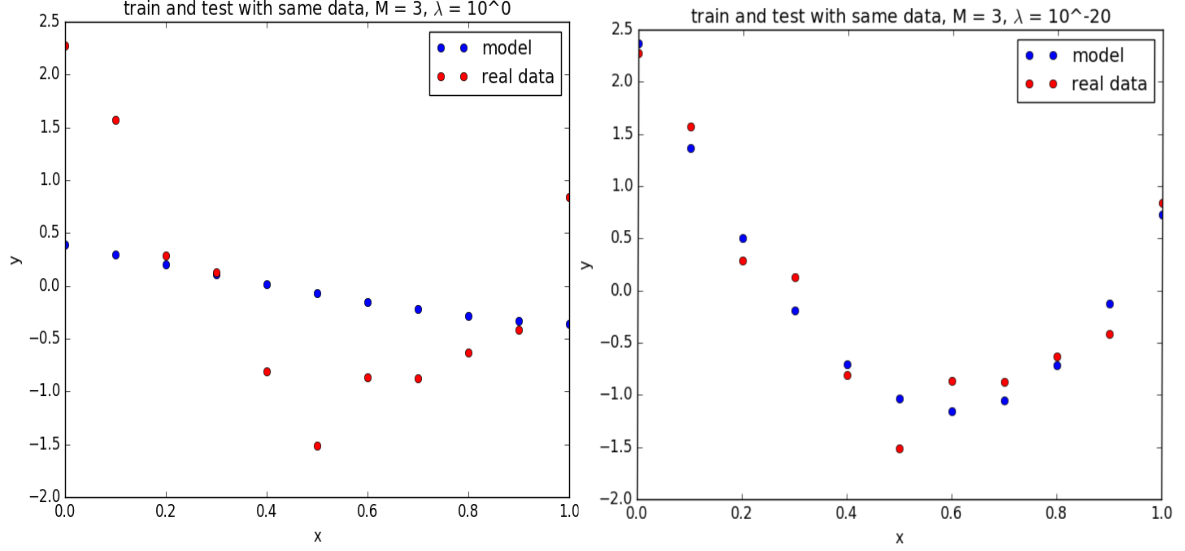
\includegraphics[width=0.9\linewidth]{figures/varying_lambda}
   \caption{The two plots show the effect of a decreasing regularization coefficient $\lambda$ on the estimator. In the left image, the regularization coefficient $\lambda = 1$. If $\lambda$ increases, it penalizes higher weights $w$ stronger, which encourages them to drive to zero. This drives the model target vector $y$ to converge to zero as well (see left). A smaller $\lambda$ does penalize higher weights less, leaving them free to form the polynomial seen on the right. A $\lambda = 0$ would equal an estimator without regularization.}
\label{varying_lambda}
\end{figure}

\begin{figure}[!ht]
   \centering
   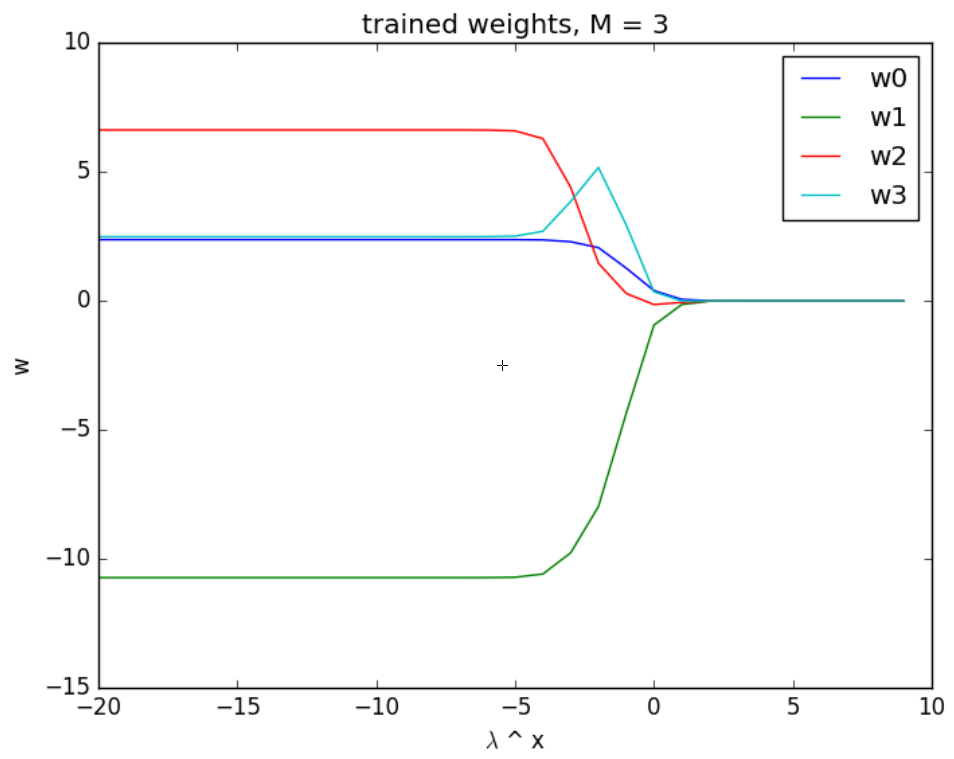
\includegraphics[width=0.8\linewidth]{figures/weights_separation}
   \caption{[x-axis is $log(\lambda)$] If $\lambda$ gets close to zero, the weight coefficients get separated (left). A $\lambda$ of exactly zero would equal the case of not having a regularization term as higher weights $w$ would not get penalized anymore. There is an intersection region around $\lambda=10^{-3}$. After the intersection region $\lambda$ becomes large and drives the weights to zero. There are $M+1$ elements of $w$ (polynomial basis with intercept).}
\label{weights_separation}
\end{figure}

\begin{figure}[!ht]
   \centering
   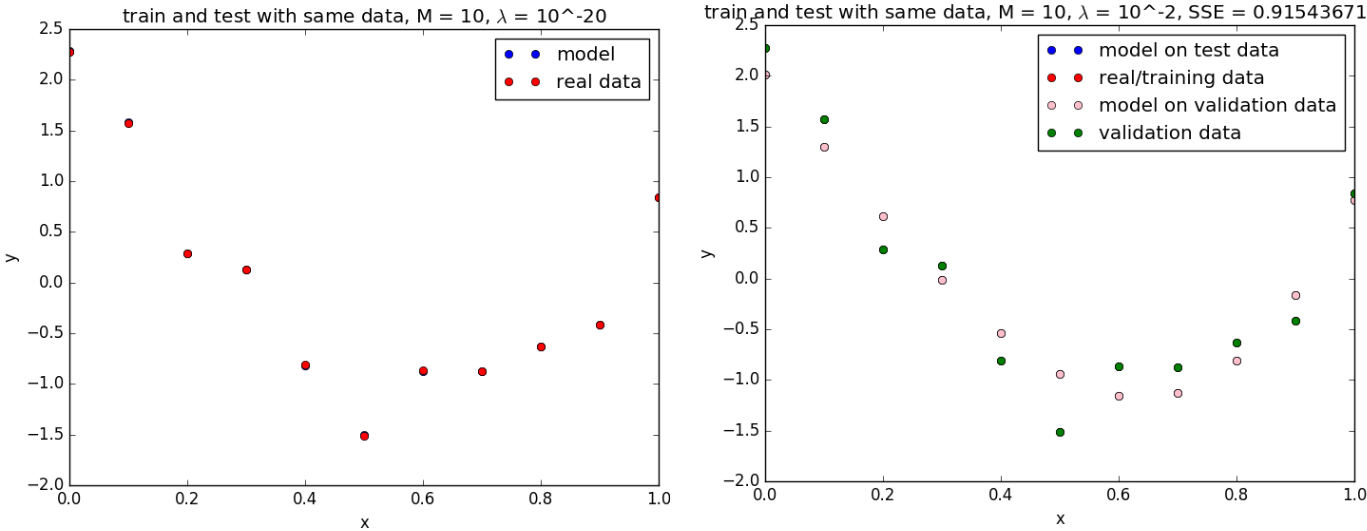
\includegraphics[width=0.9\linewidth]{figures/ridge_high_dim}
   \caption{This plot shows how complex models, represented by a the polynomial feature map $\phi$ of order $M=10$ overfit the data with linear regression (left, where $\lambda \approx 0$). The quadratic regularizor penalizes the high weights and thereby achives to estimate the training data well (right, $SEE \approx 0.92$). Fig. \ref{varying_lambda} in comparison, shows a cubic polynomial feature map. Both, linear and ridge regression have performed comparibly well on low-order models.}
\label{ridge_him_dim}
\end{figure}

\subsection{Training and testing on different data}
In practice, the weights of an estimator are trained on a training dataset, the hyperparameters are determined by a validation data and finally the performance is evaluated on the test dataset. In the earlier section, we have used one dataset for all. Now, we are given  three datasets: A, B and a validation set. Fig. \ref{trainABBA} shows the learned models and their evaluation.

\begin{figure}[!ht]
   \centering
   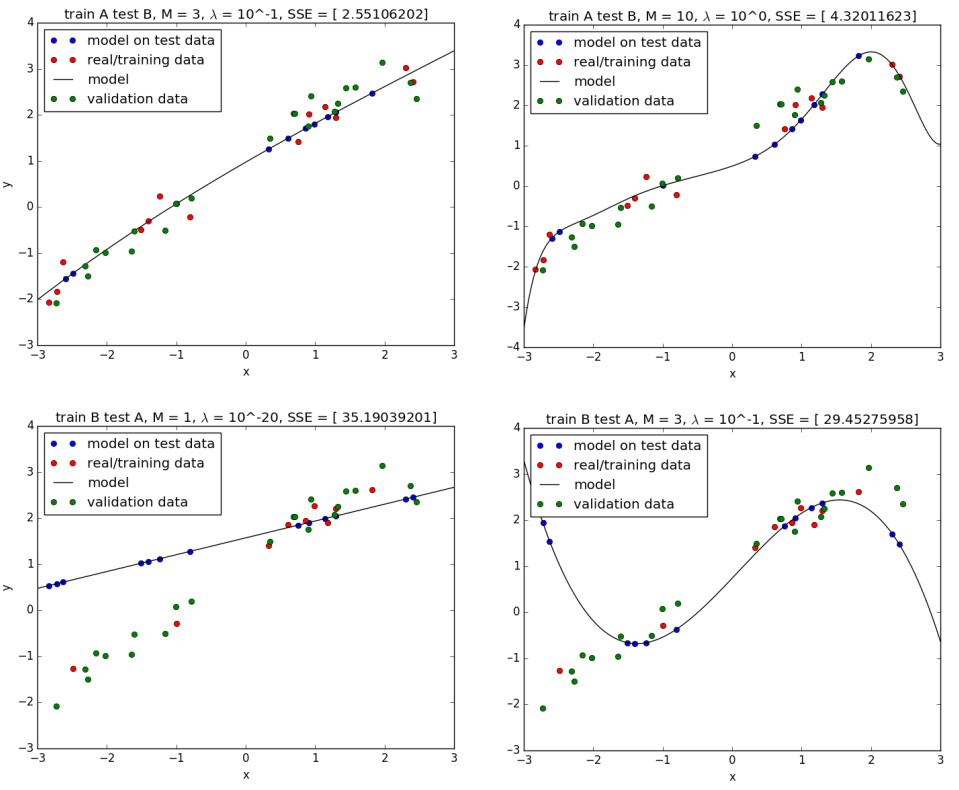
\includegraphics[width=1\linewidth]{figures/trainABBA}
   \caption{The top two figures have trained a model with dataset A, applied on the test data B and the validation dataset. The model has been tested with lower (top-left) and higher (top-right) order polynomials. The higher order one is overfitted although there we have chosen a high value for $\lambda$. Other combinations of $\lambda$ and $M$ have been evaluated according to their $SEE$. The model of degree $M=3$ and $\lambda = 0.1$ has shown the best performance with $SSE = 2.55$ and a visual graphical fit. The dataset B is characterized by one outlier value $(-2.6,3.5)$ (s. bottom plots). In the bottom plots, the model was trained with dataset B and applied to dataset A and the validation data. We can see that the outlier value has significant influence on the learned model and skews the model. We have achieved best fit ($SSE \approx 29.45$) with $M=3$ and $\lambda = 0.1$ (bottom-right). At the same time linear regression performed reasonably well with a linear curve (bottom-left). A solution to use B for training would be preprocessing the data to eliminate outlier values.}
\label{trainABBA}
\end{figure}

The sum of least squares error (SSE) is a valuable measurement index to evaluate the performance of a trained model. The SSE is given by ~\cref{eq:sse}. Varying along the hyperparameters we can find the one with the best fit on the validation data. Table \ref{table_sse} shows the influence of a varying regularization coefficient $\lambda$. For training with A, a $\lambda$ around zero shows the best results, while a training with B has the best performance with $\lambda = 1$. Further evaluation of the model can be achieved by looking at the R squared error, which will produce similar results in a scale adapted the mean of the validation dataset. 

\begin{table}[ht!]
\centering
\begin{tabular}{||c c c||}  
 \hline
 $log(\lambda)$ & $SSE_A$ & $SSE_B$ \\ [0.5ex] 
 \hline\hline
 -20 & 2.37 & 35.19 \\ 
 \hline
 -1 & 2.55 & 34.80 \\
 \hline
 0 & 4.35 & 32.10 \\
 \hline
 1 & 16.17 & 32.18 \\
 \hline
 2 & 29.54 & 62.68 \\
 \hline
 10 & 76.51 & 76.51 \\ [1ex] 
 \hline
\end{tabular}
\caption{Effect on $\lambda$ on the sum of least squares error $SSE$ on model trained with A and B and compared to validation dataset. A polynomial of $M=3$ and $M=1$ has been used for training with A and B, respectively.}
\label{table_sse}
\end{table}

\section{Sparsity and Lasso}
In ridge regression we have used a quadratic regularizor, which corresponds to the general regularized error function \ref{regularized_error}, where $q = 2$. Least absolute shrinkage and selection operator (Lasso) uses the $L_1$ norm, $q = 1$ to compute the error. Lasso gives a sparse solution model, i.e. by increasing the $\lambda$, it drives some weight coefficients to exactly zero. In this chapter, we compare the performance of Lasso to ridge regression. 

A newly given dataset was generated by a sinoid feature vector and small noise $\epsilon$. The feature vector is given by:

\begin{equation}
\phi(x) = (x, sin(0.4\pi * 1),..., sin(0.4\pi x * 12)) \in{\rm I\!R}^{13}
\label{lasso_feature}
\end{equation}

In Fig. \ref{lasso_lambda}, we can see that $\lambda = 0.1$ leads to a sparse estimation of the weight vector $w$ and only four values remain non-zero. Visualized in 2D, Lasso drives a weight tuple into the corners of a rectangle. Ridge regression drives the weights onto the circumference of a circle (Bishop 3.1.4).

\begin{figure}[!ht]
   \centering
   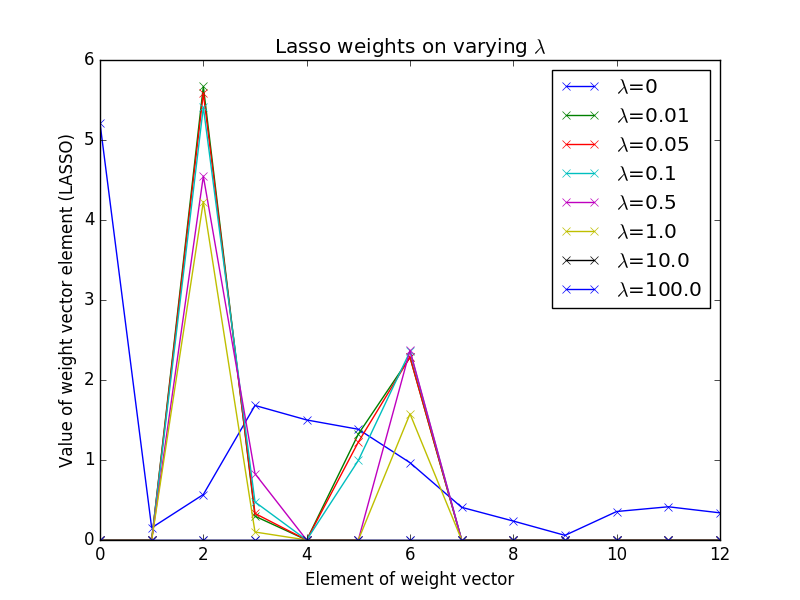
\includegraphics[width=0.9\linewidth]{figures/lasso_lambda}
   \caption{This graphs shows the relation the lasso regularization coefficient $\lambda$ to the weight vector $w$. $\lambda = 0$ equals an estimator without regularizing term. The further the $\lambda$ increases, the further the weight elements are decaying to zero. $\lambda = 0.01$ leads to a reasonable separation of the weight vector, where four elements are non-zero: $w_2, w_3, w_5$ and $w_6$}
\label{lasso_lambda}
\end{figure}

We compare the weight coefficient from Lasso with the weights from ridge and the true $w$ in Fig. \ref{lasso_weights} and visual inspection shows us that the estimated weights by lasso are very close to the true weights.

\begin{figure}[!ht]
   \centering
   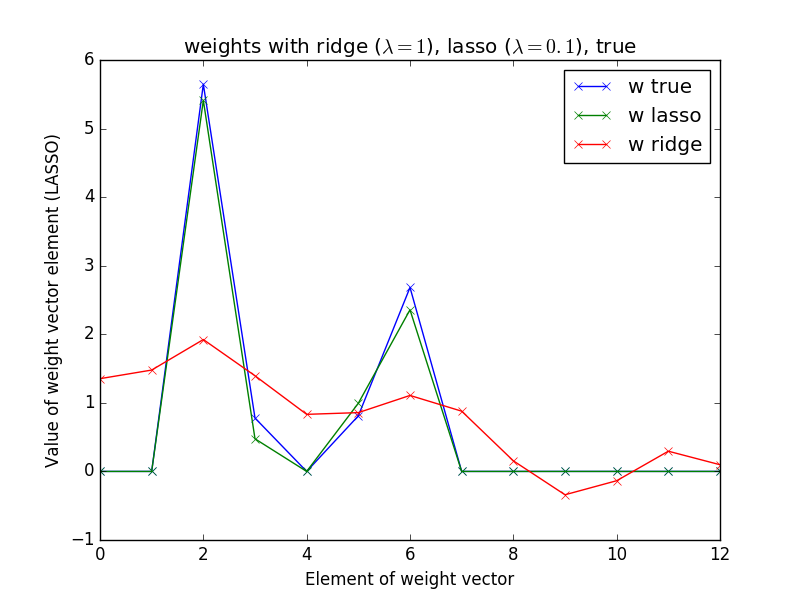
\includegraphics[width=0.9\linewidth]{figures/lasso_weights}
   \caption{This figure displays the weights from the lasso regularizor ($\lambda = 0.1$) with the estimated weights from ridge ($\lambda = 1$) and the true ones. On visual inspection, the lasso weights are very close to the true weights. All elements of the lasso weight vector have decayed to zero, such that only four non-zero elements remain. The weights from ridge regression differ strongly from the true weights and no weights are zero.}
\label{lasso_weights}
\end{figure}

In~\cref{regularizor_comparison}, we use the learned weights of ridge, lasso and the true ones onto our validation dataset. This gives us knowledge about the fit of the estimator on the real data.
Based on the smooth plot in~\cref{regularizor_comparison} and the low SSE in~\cref{table:sse_weights}, Lasso seems to generate the best model of this dataset. 
 
\begin{table}[ht!]
\centering
\begin{tabular}{||c c c c||}  
 \hline
 \ & $SSE_{val}$ & $SSE_{test}$ & $SSE_{train}$ \\ [0.5ex] 
 \hline\hline
 Lasso & 1.13 & 1.39 & 0.19 \\ 
 \hline
 Ridge & 4.03 & 7.50 & 1.70 \\
 \hline
 True & 0.41 & 0.39 & 0.25 \\[1ex] 
 \hline
\end{tabular}
\caption{This tables compares the estimators according to their sum of least squares error. We see that Lasso performs better than ridge on the validation and teh test dataset. I would not be useful to select an estimator by only looking on its performance on the trained data, as an overfitted model could achieve an error $SSE_{train}=0$. In comparison to the true data, we see that Lasso performs reasonably well.}
\label{table:sse_weights}
\end{table}

\begin{figure}[!ht]
   \centering
   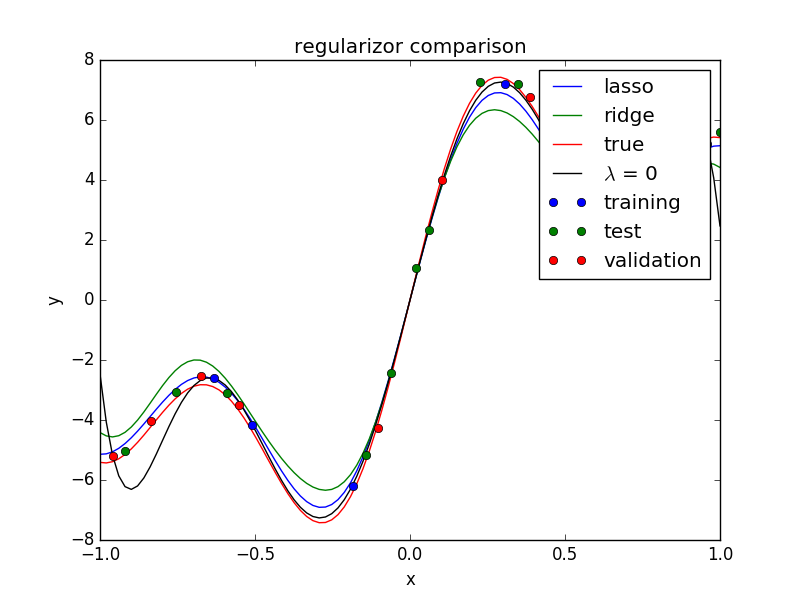
\includegraphics[width=0.9\linewidth]{figures/regularizor_comparison}
   \caption{In the plot, we have compared the performance the learned models from Lasso, ridge and linear regression ($\lambda = 0$) with the true sinoid function. The used weights are the ones displayed in~\cref{lasso_weights}. The plot also shows the used training, test and validation datasets. We can observe, that the model for the true weights and lasso weights is visually very close to the validation and test dataset. This observation gets confirmed by Table~\cref{table:sse_weights}, in which we have analysed the $SSE$ of the estimators. For this data we would select the Lasso estimator for evaluating a test dataset. The datapoints of the validation data do not fit onto the true sinoid curve, because they have been generated by adding small random noise.}
\label{regularizor_comparison}
\end{figure}


\section{Conclusion}
We have given provided a look into gradient descent, linear basis function regression, ridge regression, sparsity and LASSO. Different datasets, weights and hyperparameters have been tested and compared regarding their performance.
%\section{MNIST Dataset} \label{sec:prob4}
In this section, we use each of the algorithms to classify handwritten digits from the MNIST dataset.

\subsection{Part 1}
The MNIST dataset contains labeled, handwritten digits.
We split the dataset into multiple classification tasks, shown in the first column of~\cref{table_4_1}.
We also split it into training, validation, and testing sets.

We follow the typical procedure: train with many hyperparameters (C for $L_1$, $L_2$ for LR, and C for SVM), choose the hyperparameters that maximize performance on the validation set with lowest model complexity (low C), and report performance on the test set for the best hyperparameters.

The two classifiers here, Logistic Regression and Linear SVM, perform similarly on each classification task.
For all tasks, the training accuracy was better than the testing accuracy, as expected.

Normalization of the data did not make a large difference ($<\pm 1\%$) for these classifiers, and results presented are for non-normalized data.
The only significant difference after normalization was the size of regularization constant $C$; in all cases, normalization caused the optimal $C$ value to increase by a few orders of magnitude.
This is likely because the size of the data elements decreased, so the size of the learned weight vector increased, meaning a smaller regularization cost had to be applied for the same effect.

A couple misclassified digits are shown in~\cref{fig:misclassified}.
Some handwriting is very difficult even for humans to classify, so it makes sense that our learned classifiers are not perfect.

\begin{figure}\label{fig:misclassified}
    \centering
    \begin{subfigure}[b]{0.5\columnwidth}
        \centering
        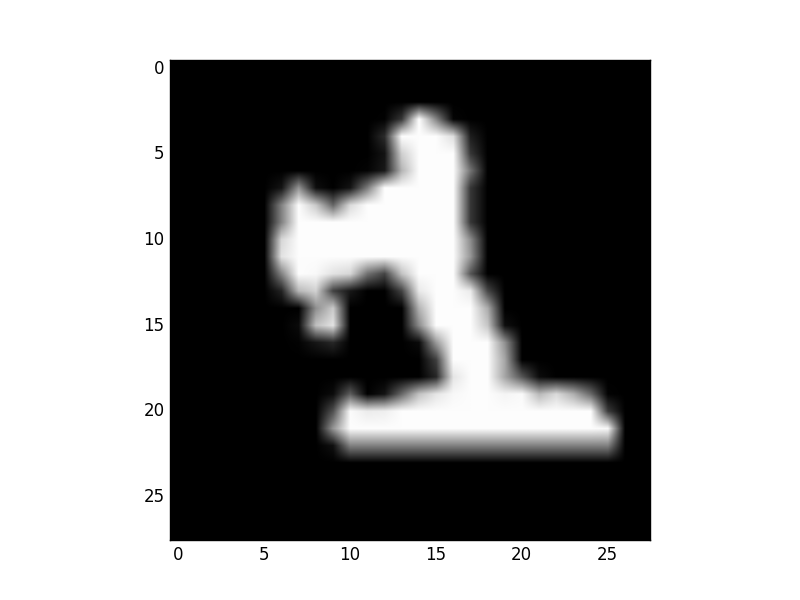
\includegraphics[height=1.2in]{figures/4_1_bad1}
        \caption{Misclassified 1}
    \end{subfigure}%
    ~ 
    \begin{subfigure}[b]{0.5\columnwidth}
        \centering
        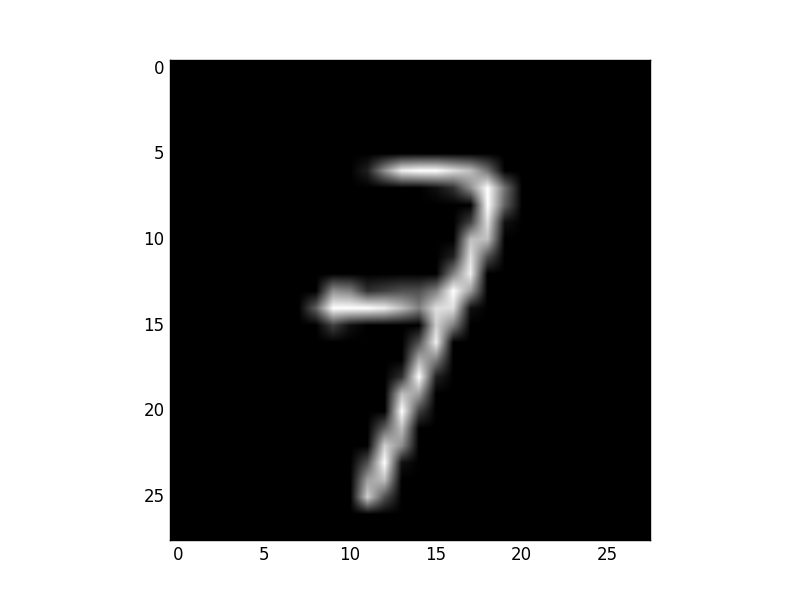
\includegraphics[height=1.2in]{figures/4_1_bad7}
        \caption{Misclassified 7}
    \end{subfigure}
    \caption{The MNIST dataset has some ambiguous entries, in accordance with real human handwriting, that are difficult to classify correctly.}
\end{figure}

\begin{table}[ht!]
\centering
\begin{tabular}{||c c c c c||}  
 \hline
 Dataset & LR Tr. & LR Test & SVM Tr & SVM Test \\ [0.3ex] 
 \hline\hline
 1 vs. 7 & 100.0 & 98.3 ($C=1$) & 100.0 & 98.7 ($C=0.2$) \\ 
 \hline
 3 vs. 5 & 100.0 & 93.3 ($C=60$) & 100.0 & 94.7 ($C=0.02$) \\ 
 \hline
 4 vs. 9 & 100.0 & 94.7 ($C=2$) & 100.0 & 94.7 ($C=0.02$) \\ 
 \hline
 odds vs. evens & 92.9 & 89.0 ($C=0.1$) & 93.9 & 89.2 ($C=0.02$) \\ 
 \hline
\end{tabular}
\caption{Accuracy of LR and Linear SVM on MNIST datasets.}
\label{table_4_1}
\end{table}

\subsection{Part 2}
Next, we applied the Gaussian RBF SVM classifier on the MNIST dataset for the same binary classification tasks.
Again, there are two parameters, $C$ (regularization) and $\gamma$ (bandwidth) that must be tuned with the validation set.
It is difficult to tune these two in parallel, especially without a method of visualizing the dataset, as was possible in the simple 2D data case.
Our approach was to train of each parameter in the range $[10^{-5}, 10^{-4}, ..., 10^{5}]$, and then compare accuracy on the validation set.
Many models had a validation accuracy of 99\%, so for these, the least complex model (low $\gamma$, low $C$).
Even so, it's very hard to select the best model because the relative importance of $C$ and $\gamma$'s size is not obvious (i.e. is a low $\gamma$ and high $C$ preferable to a high $\gamma$ and low $C$?).
The two are related to some extent; we observed roughly that an increase in order of magnitude of $\gamma$ decreases the $C$ for maximum validation accuracy, by an order of magnitude as well.
Also, $\gamma>1$ always has poor validation accuracy ($<60\%$) regardless of $C$.

The choice of $C$, $\gamma$, and training and test accuracy are shown in~\cref{table_4_2}.
Even with the poor choice of parameters in the stated range, validation accuracy was often around 70-80\%, so the classifier would not be completely useless.
For each classification task, the chosen hyperparameters are listed in~\cref{table_4_2}'s rightmost column.



[todo: compare rbf to linear classifiers]

\begin{table}[ht!]
\centering
\begin{tabular}{||c c c c||}  
 \hline
 Dataset & Tr. Acc & Test Acc & $C, \lambda$ \\ [0.3ex] 
 \hline\hline
 1 vs. 7 & 100.0 & 99.0 & 1, 0.01 \\ 
 \hline
 3 vs. 5 & 100.0 & 97.0 & 100, 0.001 \\ 
 \hline
 4 vs. 9 & 100.0 & 95.0 & 10, 0.001 \\ 
 \hline
 odds vs. evens & 100.0 & 97.2 & 1, 0.01 \\ 
 \hline
\end{tabular}
\caption{Accuracy of Gaussian RBF SVM classifier on MNIST datasets.}
\label{table_4_2}
\end{table}

\subsection{Part 3}
[todo]


%\listofchanges

%\balance

% \addtolength{\textheight}{-12cm} % This command serves to balance the column lengths
% on the last page of the document manually. It shortens
% the textheight of the last page by a suitable amount.
% This command does not take effect until the next page
% so it should come on the page before the last. Make
% sure that you do not shorten the textheight too much.

%%%%%%%%%%%%%%%%%%%%%%%%%%%%%%%%%%%%%%%%%%%%%%%%%%%%%%%%%%%%%%%%%%%%%%%%%%%%%%%%



%%%%%%%%%%%%%%%%%%%%%%%%%%%%%%%%%%%%%%%%%%%%%%%%%%%%%%%%%%%%%%%%%%%%%%%%%%%%%%%%



%%%%%%%%%%%%%%%%%%%%%%%%%%%%%%%%%%%%%%%%%%%%%%%%%%%%%%%%%%%%%%%%%%%%%%%%%%%%%%%%
% \section*{Acknowledgment}
% This work is supported by Ford Motor Company.
%%%%%%%%%%%%%%%%%%%%%%%%%%%%%%%%%%%%%%%%%%%%%%%%%%%%%%%%%%%%%%%%%%%%%%%%%%%%%%%%
%\clearpage
\balance
% \bibliographystyle{IEEEtran} 
% %\bibliographystyle{unsrt} 
% \bibliography{biblio}
% %\balance
\end{document}
%\grid
